%--------------------------------------------------------------------
% NE 155 (intro to numerical simulation of radiation transport)
% Spring 2017

% formatting
\documentclass[12pt]{article}
\usepackage[top=1in, bottom=1in, left=1in, right=1in]{geometry}

\usepackage{setspace, multicol}
\onehalfspacing

\setlength{\parindent}{0mm} \setlength{\parskip}{1em}


% packages
\usepackage{amssymb}
%% The amsthm package provides extended theorem environments
\usepackage{amsthm}
\usepackage{epsfig}
\usepackage{times}
\renewcommand{\ttdefault}{cmtt}
\usepackage{amsmath}
\usepackage{graphicx} % for graphics files

% Draw figures yourself
\usepackage{tikz} 

% The float package HAS to load before hyperref
\usepackage{float} % for psuedocode formatting
\usepackage{xspace}

% from Denovo methods manual
\usepackage{mathrsfs}
\usepackage[mathcal]{euscript}
\usepackage{color}
\usepackage{array}

\usepackage[pdftex]{hyperref}

\newcommand{\nth}{n\ensuremath{^{\text{th}}} }
\newcommand{\ve}[1]{\ensuremath{\mathbf{#1}}}
\newcommand{\macro}{\ensuremath{\Sigma}}
\newcommand{\vOmega}{\ensuremath{\hat{\Omega}}}

\newcommand{\Macro}{\ensuremath{\Sigma}}


\newcommand{\cc}[1]{\ensuremath{\overline{#1}}}
\newcommand{\ccm}[1]{\ensuremath{\overline{\mathbf{#1}}}}


%--------------------------------------------------------------------
%--------------------------------------------------------------------
\begin{document}
% Iterative methods
The \textbf{fixed-point} iterative process and associated error are (where $\rho(\ve{P})$ is the spectral radius of $\ve{P}$.):
\[\vec{x}^{(0)} = \text{ arbitrary}\:; \qquad
\vec{x}^{(k+1)} = \ve{P}\vec{x}^{(k)} + \tilde{\vec{b}} \]
\[\vec{e}^{(k+1)} = \ve{P}\vec{e}^{(k)}\:; 
 \qquad ||\vec{e}^{(k+1)}|| \leq ||\ve{P}^{k+1}||\: ||\vec{e}^{(0)}||\:;
 \qquad || \ve{P}^k || \approx \rho^k (\ve{P})\]
%
To reduce error by a factor of $\epsilon$, it takes $k \approx \frac{\log(\epsilon)}{\log(\rho(\ve{P}))}$ iterations. 
%
    \begin{table}[h!]
    \centering
      \begin{tabular}{| c | c | }
        \hline
        Richardson & Jacobi \\ \hline
        \hline
        $(\ve{I} - \omega^{(k)}\ve{A})\vec{x}^{(k)} + \omega^{(k)}\vec{b}$   &  
        $ \ve{D}^{-1}(\ve{D} - \ve{A})\vec{x}^{(k)} + \ve{D}^{-1}\vec{b}$  \\
        \hline  
        GS & SOR \\ \hline
        $ (\ve{D} + \ve{L})^{-1} \bigl[-\ve{U} \vec{x}^{(k)} + \vec{b}\bigr] $ &  
        $ (\ve{D} + \omega \ve{L})^{-1} \Bigl( [(1-\omega)\ve{D} - \omega \ve{U}] \vec{x}^{(k)} + \omega\vec{b} \Bigr)$ \\
        \hline        
      \end{tabular}
      \caption{$\vec{x}^{(k+1)}$ for several iterative methods}
      \label{tab:delayedneutrons}
    \end{table}
%\begin{align*}
%\text{Richardson} \qquad &\vec{x}^{(k+1)} = (\ve{I} - \omega^{(k)}\ve{A})\vec{x}^{(k)} + \omega^{(k)}\vec{b}\:;
% \qquad x^{(k+1)}_i =  x^{(k)}_i - \omega^{(k)} \sum_{j=1}^{n} a_{ij}x_j^{(k)} + \omega^{(k)} b_i \\
%%
%\text{Jacobi} \qquad & \vec{x}^{(k+1)} = \ve{D}^{-1}(\ve{D} - \ve{A})\vec{x}^{(k)} + \ve{D}^{-1}\vec{b}\:;
%  \qquad x^{(k+1)}_i = \frac{1}{a_{ii}}(b_i - \sum_{j=1}^{i-1} a_{ij} x_j^{(k)} - \sum_{j=i+1}^{n} a_{ij} x_j^{(k)})\\
%%
%\text{GS} \qquad &  x^{(k+1)}_i = \frac{1}{a_{ii}}(b_i - \sum_{j=1}^{i-1} a_{ij} x_j^{(k+1)} - \sum_{j=i+1}^{n} a_{ij} x_j^{(k)})\\
%%
%\text{SOR} \qquad & x^{(k+1)}_i = (1-\omega)x_i^{(k)} + \frac{\omega}{a_{ii}}(b_i - \sum_{j=1}^{i-1} a_{ij} x_j^{(k+1)} - \sum_{j=i+1}^{n} a_{ij} x_j^{(k)}) 
%\end{align*}
%

\vspace*{-1em}
\textbf{condition number} of a matrix $\mathbf{A}$ is defined as $\kappa(\mathbf{A}) = ||\mathbf{A}|| \text{ }||\mathbf{A}^{-1}||$.
%
If the 2-norm is used, then $||\mathbf{A}||_{2} = \sigma_{1}$, $||\mathbf{A}^{-1}||_{2} = 1 / \sigma_{m}$, and $\kappa_{2}(\mathbf{A}) = \sigma_{1} / \sigma_{m}$; $\sigma_{m}$ is the $m$th singular value of $\ve{A}$. %If $\mathbf{A}$ is singular, its condition number is infinity. 

Let $\ve{G}$ be a non-singular \textbf{preconditioner}, then $\ve{A}\vec{x}=\vec{b}$ can be transformed as $\ve{G}^{-1}\ve{A}x = \ve{G}^{-1}b$.

% finite difference
\textbf{Finite Difference} for the DE in \underline{1D} we use central difference for the derivative: 
\[-\phi_{i-1} + \bigl(2 + \frac{h^2}{L^2}\bigr)\phi_i - \phi_{i+1} = h^2 \frac{S_{0,i}}{D} \qquad i = 1, 2, \dots, n-1 \qquad L \equiv \sqrt{\frac{D}{\Sigma_a}}\]

In \underline{2D} we use a 5-point stencil and use central in each dimension for the derivative, giving
\[ \nabla^2 \phi_{i,j} = \frac{\phi_{i+1,j} + \phi_{i-1,j} + \phi_{i,j+1} + \phi_{i,j-1} - 4\phi_{i,j}}{h^2}\]


% finite volume
\textbf{Finite Volume} for the DE in \underline{1D} uses this grid 
%
\begin{multicols}{2}
\begin{center}
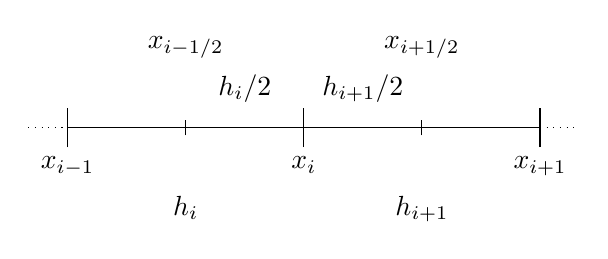
\begin{tikzpicture}
\draw[dotted] (0,0)--(0.5,0);
\draw (0.5,0)--(3.5,0);
\draw (.5,-.25)--(.5,.25);
\draw (2,-.1)--(2,.1);
\draw (3.5,-.25)--(3.5,.25);
\draw (0.5,0)--(6.5,0);
\draw[dotted] (6.5,0)--(7,0);
\draw (.5,-.25)--(.5,.25);
\draw (5,-.1)--(5,.1);
\draw (6.5,-.25)--(6.5,.25);
\node[below] at (.5,-.25) {$x_{i-1}$};
\node[below] at (6.5,-.25) {$x_{i+1}$};
\node[below] at (3.5,-.25) {$x_i$};
\node[above] at (2, 0.75) {$x_{i-1/2}$};
\node[above] at (5, 0.75) {$x_{i+1/2}$};
\node[below] at (2, -.75) {$h_{i}$};
\node[below] at (5, -.75) {$h_{i+1}$};
\node[above] at (4.25, .2) {$h_{i+1}/2$};
\node[above] at (2.75, .2) {$h_{i}/2$};
\end{tikzpicture}
\end{center}
\columnbreak
The physics values are defined in each cell (cell-centered) and the flux and source are defined at the mesh points (edge-centered.\\
We integrate the DE in each cell from $x_{i-1/2}$ to $x_{i+1/2}$. At the boundaries we apply the BCs as appropriate to get the $i=0$ and $i=n$ equations.
\end{multicols}


The \underline{2D} version uses a 2D stencil (not needed for exam). The physics values are again defined in each cell (cell-centered) and the flux and source are defined at the mesh points (edge-centered.\\
We again integrate over the partial cell, which is now in two dimensions: $x_{i-1/2}$ to $x_{i+1/2}$ and $y_{j-1/2}$ to $y_{j+1/2}$.\\
We use Gauss Theorem for the streaming term: $-\int_V d\vec{r}\:\bigl[\nabla \cdot \bigl(D(\vec{r})\nabla \phi(\vec{r})\bigr)\bigr] = \int_S d\vec{S} \:D(\vec{r})\frac{\partial}{\partial \hat{n}}\phi(\vec{r})$.

% Criticality
\textbf{Critical/eigenvalue} equations have the addition of $k$, allowing us to adjust the equation such that the rhs of the DE becomes $\frac{1}{k}\nu \Sigma_f(x) \phi(x)$. \\
This means the rhs of our FD or FVM matrix formulation contains flux instead of only a fixed source. 
\vspace*{-1.25em}
\begin{align*}
A &= -\frac{d}{dx}D(x)\frac{d}{dx} + \Sigma_a(x) \qquad F = \nu\Sigma_f(x) \qquad k = \frac{\text{total production rate}}{\text{total loss rate}}\\
%
\ve{A} &\vec{\phi}^{(m+1)} = \frac{1}{k^{(m)}}\ve{F}\vec{\phi^{(m)}} \qquad 
k^{(m+1)} = \frac{\int_0^{\tilde{a}} F \vec{\phi}^{(m+1)}(x)dx}{\frac{1}{k^{(m)}}\int_0^{\tilde{a}} F \vec{\phi}^{(m)}(x)dx}
\end{align*}

\vspace*{-1.5em}
We also add an eigenvalue solver method, like Power Iteration. This uses the idea that \\$\vec{v}_0 = \gamma_1 \vec{x}_1 + \gamma_2 \vec{x}_2 + \cdots + \gamma_n \vec{x}_n$, where $\vec{x}_{j}$ is the $j$th eigenvector and $\gamma_{j}$ is some constant.

% PRKE
\textbf{Delayed neutrons} let us deal with time variation. $\beta$ fraction of the total neutrons released from fission are delayed. We use $\rho =\mbox{reactivity} = \frac{k-1}{k}$, and $l$ is mean neutron lifetime. 
\begin{align*}
  n(t) &= n_0e^{\frac{(k-1)t}{l}}\:; \qquad T = \text{reactor period} = \frac{l}{k-1}\\
  &\phi(r,t) = vn(t)\psi_1(r)\:; \qquad
  \hat{C}_i(r,t) = C_i(t)\psi_1(r)\\
  &\text{where $\psi_1$ is the fundamental mode solution of }   \nabla^2\psi_n + B_g^2\psi_n = 0%\\
  %
%  \frac{1}{v}\frac{\partial \phi(r,t)}{\partial t} &- \nabla D(r,t) \nabla \phi(r,t) + \
%  \Sigma_a(r,t)\phi(r,t) = (1-\beta)\nu\Sigma_F(r,t)\phi(r,t) + \
%  \sum_{i=1}^6\lambda_i\hat{C}_i(r,t)
\end{align*}
\textbf{PRKE}
\vspace*{-1em}
\begin{align*}
  \frac{dn(t)}{dt} = \frac{\rho(t)-\beta}{\Lambda}n(t) + \sum_{i=1}^{6}\lambda_iC_i(t) \:; \qquad
  \frac{dC_i(t)}{dt} = \frac{\beta_i}{\Lambda}n(t) - \lambda_i C_i(t)
 \end{align*}
 
 \vspace*{-1.5em}
$C_i(t)$ = delayed neutron concentration from ith precursor; $\Lambda$ = effective n lifetime = $(v\nu\Sigma_F)^{-1}$.

\textbf{Runge Kutta} methods use stages to avoid higher order derivates to get better accuracy. Two stage:
\vspace*{-.5em}
\[U^{n+1/2} = U^n + \frac{1}{2}kf(U^n)\qquad U^{n+1} = U^n + kf(U^{n+1/2}) \qquad U^{n+1} = U^n + kf(U^n + \frac{1}{2}kf(U^n))\]

\textbf{Monte Carlo} uses random numbers, sampling rules, tallies, and \underline{statistics}
\begin{align*}
\mu &= E(x) = \int x f(x) dx \:;  \qquad \bar{x} = \frac{1}{N}\sum_{i=1}^N x_i \quad \lim_{N \to \infty} \bar{x} \rightarrow \mu \\
%
\sigma^2 &= E(x^2) - \mu^2 \:; \qquad S_x^2 \approx \bar{x^2} - \bar{x}^2\:; \qquad S_{\bar{x}}^2 = \frac{S_x^2}{N}
\end{align*}
%
\begin{align*}
    p\left\lbrace a \leq x \leq b \right\rbrace &= \int_a^b p(x)dx\:; \qquad    p(x)  \geq 0 \:; \qquad    \int_{-\infty}^{\infty} p(x)dx = 1\\
    %
    p(x = x_k) &= p_k \equiv p(x_k)\:,  k = 1, \dots, N \:; \qquad  p_k  \geq 0\:; \qquad \sum_{k=1}^N p_k = 1\\
    % 
    P\left\lbrace x' \leq x \right\rbrace &= P(x) = \int_{-\infty}^x p(x')dx'\ \:; \qquad P(-\infty) = 0 \:,\quad P(\infty) = 1\\
    %
    P\left\lbrace x' \leq x \right\rbrace &= P_k \equiv P(x_k) = \sum_{j=1}^k p_j\:, k = 1, \dots, N \:; \qquad P_0 = 0 \:,\quad P_N = 1
\end{align*}
Deal with \underline{normalization} using $p(x) = \frac{g(x)}{G(\infty)}$, where $p(x)$ is the numerical PDF, $g(x)$ is the physical PDF, and $G(x)$ is the physical CDF.

With \underline{rejection sampling}, create $g(x)\geq p(x)$ for all $x$; Generate pair of random variables, $(\xi, \eta)$; $x' = G^{-1} (\xi)$; If $\eta < p(x')/g(x')$, accept $x'$;  Else, reject $x'$.

Probability of \underline{distance to collision}
    \begin{align*}
    p_c(s) &= \Sigma_t(s) e^{-\Sigma_t(s) s} ds \\
    P_c(n) &= \int_0^s \Sigma_t(s) e^{-\Sigma_t(s) s'}ds' = -e^{-\Sigma_t(s) s'} |_0^s = 1 - e^{-\Sigma_t(s) s}
  \end{align*}
After a collision, which nuclide from $p_i = \frac{\Sigma_{t,j}}{\Sigma_t}$ and which reaction from $p_x = \frac{\Sigma_{x,j}}{\Sigma_{t,j}}$.
  
In scattering, ihe new direction is $\bigl(\sin(\phi) \cos(\theta), \sin(\phi) \sin(\theta), \cos(\theta)\bigr) =\\ \bigl(\sqrt{1 - \mu^2} \cos(\theta),  \sqrt{1 - \mu^2} \sin(\theta), \mu \bigr)$.

\end{document}